\documentclass[a4paper,11pt]{report}
\usepackage{chuan_math_gkt}
\usetikzlibrary{angles,quotes,intersections,patterns,decorations.pathreplacing}
\chuanexamsetup

\begin{document}
\examfontsize

\examsecret{绝密$\bigstar$启用前}

\examtitle{2022年普通高等学校招生全国统一考试（新高考I卷）}{数\quad 学}

\noticetitle
\begin{examnotice}
\item 答卷前，考生务必将自己的姓名、准考证号填写在答题卡上. 
\item 回答选择题时，选出每小题的答案后，用铅笔把答题卡上对应题目的答案标号涂黑. 如需改动，用橡皮擦干净后，再选涂其他答案标号. 回答非选择题时，将答案写在答题卡上. 写在本试卷上无效. 
\item 考试结束后，将本试卷和答题卡一并交回. 
\end{examnotice}

\examsection{一、选择题：本题共8小题，每小题5分，共40分. 在每小题给出的四个选项中，只有一项是符合题目要求的. }
\begin{examquestions}
\item 若集合 $M=\{x\mid \sqrt x<4\}$，$N=\{x\mid 3x\geq1\}$，则 $M\cap N=$
\fourchoices{$\{x\mid 0\leq x<2\}$}{$\left\{x\mid \dfrac13\leq x<2\right\}$}{$\{x\mid 3\leq x<16\}$}{$\left\{x\mid \dfrac13\leq x<16\right\}$}
\item 若 $\mathrm{i}(1-z)=1$，则 $z+\overline z=$
\fourchoices{$-2$}{$-1$}{$1$}{$2$}
\item 在 $\triangle ABC$ 中，点 $D$ 在边 $AB$ 上，$BD=2DA$. 记 $\overrightarrow{CA}=\vec m$，$\overrightarrow{CD}=\vec n$，则 $\overrightarrow{CB}=$
\fourchoices{$3\vec m-2\vec n$}{$-2\vec m+3\vec n$}{$3\vec m+2\vec n$}{$2\vec m+3\vec n$}
\item 南水北调工程缓解了北方一些地区水资源短缺问题，其中一部分水蓄入某水库. 已知该水库水位为海拔 $1485\mathrm{m}$ 时，相应水面的面积为 $140.0\mathrm{km}^2$；水位为海拔 $1575\mathrm{m}$ 时，相应水面的面积为 $180.0\mathrm{km}^2$，将该水库在这两个水位间的形状看作一个棱台，则该水库水位从海拔 $1485\mathrm{m}$ 上升到 $1575\mathrm{m}$ 时，增加的水量约为（$\sqrt7\approx2.65$）
\fourchoices{$1.0\times10^9\mathrm{m}^3$}{$1.2\times10^9\mathrm{m}^3$}{$1.4\times10^9\mathrm{m}^3$}{$1.6\times10^9\mathrm{m}^3$}
\item 从2至8的7个整数中随机取2个不同的数，则这2个数互质的概率为
\fourchoices{\tallchoice{$\dfrac16$}}{\tallchoice{$\dfrac13$}}{\tallchoice{$\dfrac12$}}{\tallchoice{$\dfrac23$}}
\item 记函数 $f(x)=\sin\left(\omega x+\dfrac\pi4\right)+b(\omega>0)$ 的最小正周期为 $T$. 若 $\dfrac{2\pi}{3}<T<\pi$，且 $y=f(x)$ 的图象关于点 $\left(\dfrac{3\pi}{2},2\right)$ 中心对称，则 $f\left(\dfrac\pi2\right)=$
\fourchoices{$1$}{\tallchoice{$\dfrac32$}}{\tallchoice{$\dfrac52$}}{$3$}
\item 设 $a=0.1e^{0.1}$，$b=\dfrac19$，$c=-\ln0.9$，则
\fourchoices{$a<b<c$}{$c<b<a$}{$c<a<b$}{$a<c<b$}
\item 已知正四棱锥的侧棱长为 $l$，其各顶点都在同一球面上. 若该球的体积为 $36\pi$，且 $3\leq l\leq3\sqrt3$，则该正四棱锥体积的取值范围是
\fourchoices{\tallchoice{$\left[18,\dfrac{81}{4}\right]$}}{\tallchoice{$\left[\dfrac{27}{4},\dfrac{81}{4}\right]$}}{\tallchoice{$\left[\dfrac{27}{4},\dfrac{64}{3}\right]$}}{$[18,27]$}
\end{examquestions}
\examsection{二、选择题：本题共4小题，每小题5分，共20分. 在每小题给出的选项中，有多项符合题目要求. 全部选对的得5分，部分选对的得2分，有选错的得0分. }
\begin{examquestions}[start=9]
\item 已知正方体 $ABCD-A_1B_1C_1D_1$，则
\twochoices{直线 $BC_1$ 与 $DA_1$ 所成的角为 $90^\circ$}{直线 $BC_1$ 与 $CA_1$ 所成的角为 $90^\circ$}{直线 $BC_1$ 与平面 $BB_1D_1D$ 所成角为 $45^\circ$}{直线 $BC_1$ 与平面 $ABCD$ 所成的角为 $45^\circ$}
\item 已知函数 $f(x)=x^3-x+1$，则
\twochoices{$f(x)$ 有两个极值点}{$f(x)$ 有三个零点}{点 $(0,1)$ 是曲线 $y=f(x)$ 的对称中心}{直线 $y=2x$ 是曲线 $y=f(x)$ 的切线}
\item 已知 $O$ 为坐标原点，点 $A(1,1)$ 在抛物线 $C:x^2=2py(p>0)$ 上，过点 $B(0,-1)$ 的直线交 $C$ 于 $P,Q$ 两点，则
\twochoices{$C$ 的准线为 $y=-1$}{直线 $AB$ 与 $C$ 相切}{$|OP|\cdot|OQ|>|OA|^2$}{$|BP|\cdot|BQ|>|BA|^2$}
\item 已知函数 $f(x)$ 及其导函数 $f'(x)$ 的定义域均为 $\mathbb R$，记 $g(x)=f'(x)$，若 $f\left(\dfrac32-2x\right)$，$g(2+x)$ 均为偶函数，则
\twochoices{$f(0)=0$}{$g\left(-\dfrac12\right)=0$}{$f(-1)=f(4)$}{$g(-1)=g(2)$}
\end{examquestions}
\examsection{三、填空题：本题共4小题，每小题5分，共20分. }
\begin{examquestions}[start=13]
\item $\left(1-\dfrac yx\right)(x+y)^8$ 的展开式中 $x^2y^6$ 的系数为\blank（用数字作答）. 
\item 写出与圆 $x^2+y^2=1$ 和 $(x-3)^2+(y-4)^2=16$ 都相切的一条直线的方程\blank. 
\item 若曲线 $y=(x+a)e^x$ 有两条过坐标原点的切线，则 $a$ 的取值范围是\blank. 
\item 已知椭圆 $C:\dfrac{x^2}{a^2}+\dfrac{y^2}{b^2}=1(a>b>0)$，$C$ 的上顶点为 $A$，两个焦点为 $F_1,F_2$，离心率为 $\dfrac12$. 过 $F_1$ 且垂直于 $AF_2$ 的直线与 $C$ 交于 $D,E$ 两点，$|DE|=6$，则 $\triangle ADE$ 的周长是\blank. 
\end{examquestions}
\examsection{四、解答题：本题共6小题，共70分. 解答应写出文字说明、证明过程或演算步骤. }
\begin{examanswers}[start=17]
\item（10分）

记 $S_n$ 为数列 $\{a_n\}$ 的前 $n$ 项和，已知 $a_1=1$，$\left\{\dfrac{S_n}{a_n}\right\}$ 是公差为 $\dfrac13$ 的等差数列. 

\subq{（1）}{求 $\{a_n\}$ 的通项公式；}

\subq{（2）}{证明：$\dfrac1{a_1}+\dfrac1{a_2}+\cdots+\dfrac1{a_n}<2$.}
\item（12分）

记 $\triangle ABC$ 的内角 $A,B,C$ 的对边分别为 $a,b,c$，已知 $\dfrac{\cos A}{1+\sin A}=\dfrac{\sin2B}{1+\cos2B}$. 

\subq{（1）}{若 $C=\dfrac{2\pi}{3}$，求 $B$；}

\subq{（2）}{求 $\dfrac{a^2+b^2}{c^2}$ 的最小值.}
\item（12分）

如图，直三棱柱 $ABC-A_1B_1C_1$ 的体积为4，$\triangle A_1BC$ 的面积为 $2\sqrt2$. 

\noindent\begin{minipage}[t]{0.62\linewidth}
\subq{（1）}{求 $A$ 到平面 $A_1BC$ 的距离；}

\subq{（2）}{设 $D$ 为 $A_1C$ 的中点，$AA_1=AB$，平面 $A_1BC\perp$ 平面 $ABB_1A_1$，求二面角 $A-BD-C$ 的正弦值.}
\end{minipage}\hfill
\begin{minipage}[t]{0.32\linewidth}\vspace{-0.8em}\centering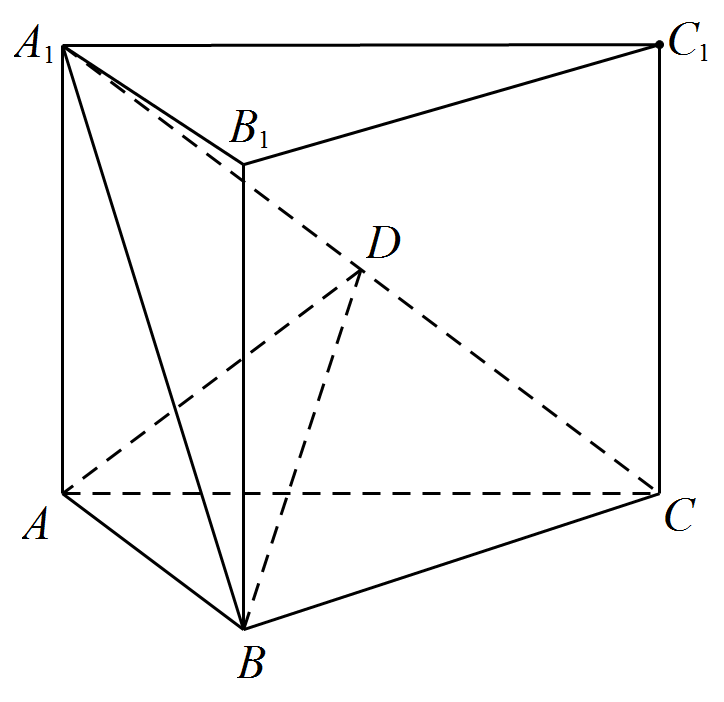
\includegraphics[width=\linewidth]{figures/2022_xgk1_q19.png}\end{minipage}
\item（12分）

一医疗团队为研究某地的一种地方性疾病与当地居民的卫生习惯（卫生习惯分为良好和不够良好两类）的关系，在已患该疾病的病例中随机调查了100例（称为病例组），同时在未患该疾病的人群中随机调查了100人（称为对照组），得到如下数据：
\begin{tightcenter}\begin{tabular}{|c|c|c|}\hline & 不够良好 & 良好\\ \hline 病例组 & 40 & 60\\ \hline 对照组 & 10 & 90\\ \hline\end{tabular}\end{tightcenter}
\subq{（1）}{能否有99\%的把握认为患该疾病群体与未患该疾病群体的卫生习惯有差异？}

\subq{（2）}{从该地的人群中任选一人，$A$ 表示事件“选到的人卫生习惯不够良好”，$B$ 表示事件“选到的人患有该疾病”. $\dfrac{P(B\mid A)}{P(\overline B\mid A)}$ 与 $\dfrac{P(B\mid\overline A)}{P(\overline B\mid\overline A)}$ 的比值是卫生习惯不够良好对患该疾病风险程度的一项度量指标，记该指标为 $R$.}

\subq{（i）}{证明：$R=\dfrac{P(A\mid B)}{P(\overline A\mid B)}\cdot\dfrac{P(\overline A\mid\overline B)}{P(A\mid\overline B)}$；}

\subq{（ii）}{利用该调查数据，给出 $P(A\mid B),P(A\mid\overline B)$ 的估计值，并利用（i）的结果给出 $R$ 的估计值. 
附 $K^2=\dfrac{n(ad-bc)^2}{(a+b)(c+d)(a+c)(b+d)}$. 
\begin{tightcenter}{\renewcommand{\arraystretch}{0.9}\begin{tabular}{|c|c|c|c|}\hline $P(K^2\geq k)$ & 0.050 & 0.010 & 0.001\\ \hline $k$ & 3.841 & 6.635 & 10.828\\ \hline\end{tabular}}\end{tightcenter}
}
\item（12分）

已知点 $A(2,1)$ 在双曲线 $C:\dfrac{x^2}{a^2}-\dfrac{y^2}{a^2-1}=1(a>1)$ 上，直线 $l$ 交 $C$ 于 $P,Q$ 两点，直线 $AP,AQ$ 的斜率之和为0. 

\subq{（1）}{求 $l$ 的斜率；}

\subq{（2）}{若 $\tan\angle PAQ=2\sqrt2$，求 $\triangle PAQ$ 的面积.}
\item（12分）

已知函数 $f(x)=e^x-ax$ 和 $g(x)=ax-\ln x$ 有相同的最小值. 

\subq{（1）}{求 $a$；}

\subq{（2）}{证明：存在直线 $y=b$，其与两条曲线 $y=f(x)$ 和 $y=g(x)$ 共有三个不同的交点，并且从左到右的三个交点的横坐标成等差数列.}
\end{examanswers}

\end{document}
